%% LyX 2.0.7 created this file.  For more info, see http://www.lyx.org/.
%% Do not edit unless you really know what you are doing.
\documentclass[oribibl]{llncs}
%\usepackage[utf8]{luainputenc}
%\setcounter{secnumdepth}{3}
%\setcounter{tocdepth}{3}
\exhyphenpenalty=10000
\hyphenpenalty=10000
\usepackage{hyperref}
\usepackage{float}
\usepackage{longtable}

\makeatletter

%%%%%%%%%%%%%%%%%%%%%%%%%%%%%% LyX specific LaTeX commands.
%% Because html converters don't know tabularnewline
%\providecommand{\tabularnewline}{\\}
%
%\makeatother

\begin{document}

\title{Structure Based Classification of Web Pages}
\author{Bharadwaj J(CS13M058) \and \\ Pankaj Kashyap(CS13M035)}
     
\institute{Dept. of CSE, IIT Madras}
\maketitle
\begin{abstract}
Given a large set of web pages in the retail domain, our aim is to
classify them into Product Pages, Product Listing Pages and Irrelevant
Pages. Several types of features can be used to classify webpages,
depending on the domain of the data. Since, we have two classes, with
similar content, viz. Products and Product Listings, we focus on using
features that exploit the structural differences between these pages
in addition to the content. Since, the irrelevant class, corresponds
to all webpages that are neither product nor listing pages, we need
to explore different options for representing them correctly, in our
training data. By training classifiers on the data obtained from a
large number of retail websites, we will experimentally prove that
our model predicts the class of any webpage accurately.
\end{abstract}

\section{Introduction}

Classifying webpages into meaningful classes, can have different benefits,
depending on the domain. One such application is to improve the efficiency
of a web crawler. A web crawler is a program, that accesses a set of
webpages. It works as follows: It starts by visiting an initial set
of webpage URLs called seeds. Once the crawler visits a webpage, it
adds all hyperlinks in that webpage to an internal list it maintains,
called the Crawler Frontier List and visits these pages. The above
operation is repeated recursively, till a termination criterion is
reached. Ideally, we would like the crawler to visit only a subset
of the webpages that can be accessed from the seeds. For this, we
can associate a classifier with the crawler and the crawler will crawl
only those pages, that belong to a particular class, and the others
can be discarded.

In our case, we have three classes of webpages, viz Product pages,
Product Listing pages and Irrelevant pages. Product pages are those
that contain detailed description of the products, their prices and
several other attributes. They are the most vital of the three, as
they are regularly updated whenever prices change, new offers are
introduced, when the product goes out of stock and several other situations.
Next in importance, are the listing pages. Many retail web sites,
have a brief description of the products in the listing page itself,
so that the customers need not open the product pages of all the products
of a particular category. This might lead to periodic changes in the
listing pages, as they have to be in sync with the corresponding product
pages. The irrelevant pages are of least significance and need not
be updated on a regular basis. These include pages such as Ads, Contact
us, Login and Account Settings etc. The website team, will prefer
to skip through these pages, while looking for product information.
Hence, by maintaining categories, the website team can easily access only those pages, that they wish to see.

There are several challenges involved in training such a classifier.
First of all, there are a huge number of retail websites available
online and hence, there is a large variation in the structure and
content of webpages across different websites. It is difficult to
find features, that are common to all retailer websites. Also, it
is difficult to obtain data for training, since we cannot be sure,
what amount of data would be sufficient to train a classifier that
will work for all types of retail webpages. The irrelevant class poses
a unique challenge as it includes all pages on the web, that do not
have product information. We need to collect data that describes all
types of irrelevant pages.

The data used for training consisted of 22801 webpages, out of which
3863 were product pages, 12354 were product listing pages and 6584
are irrelevant pages . Natural Language Toolkit was used for extracting
the features and Scikit Learn package, was used for training the classifiers.


\section{Methodology}

An array of feature extraction and training approaches were tried and compared. The final classification approach might require a combination of several different approaches. These are explained in detail, in the following sections.


\subsection{Feature Extraction}

For a html document features can be of two types: \textit{Text Features}
and \textit{Structural Features}. Several other features are also possible, but the scope of our work is restricted to these two sets of features and their hybrid combination. Text features indicate the presence
or absence of each word in the html document. Structural features
on the other hand, capture the structure of a webpage\cite{f}. These
include the number of tags, the depth of each tag, the number of children
under each tag, number of descendents of each tag etc. The structural
features themselves, might not carry much information about the webpage.
However, when combined with the text features,they are expected to
improve the results. 

The above process generates close to 7000 features. All of these might
not be useful, as most of them might contain redundant information
and several others will be common for all webpages. For example, tags
like <html>, <head> are common to all webpages and the features corresponding
to these can be safely removed. The $\chi^{2}$ feature selection
technique \cite{e} was used for selecting the best features. It calculates
$\chi^{2}$ scores for each feature and the features with top k scores
are selected. The $\chi^{2}$scores are a direct indication of the
dependence of the class label on that feature. Hence if the $\chi^{2}$
score of a feature is very less, it implies that the feature does
not contribute much in deciding the class label and hence, can be
ignored. Different values of k were tried from 100 to 2000, where
k is the number of features to be selected. For k values above 500,
there was not much improvement in performance. Hence we selected the
the top 500 features to be used in training


\subsection{Training and Testing}

Two different approaches were used for training. In the first approach,
the irrelevant webpages were treated as outliers and in the second,
they were treated as a third class.

The first approach is based on the assumption that, no amount of irrelevant
webpages is sufficient to describe the irrelevant class, as they can
be extremely diverse. For this approach, we trained One class SVMs
using Radial Basis Function kernel \cite{a}\cite{b}, on the product
and product listing datasets. Since, we need to minimize both false
positives and false negatives, the model with the highest f-measure
was considered as the best model and its results are tabulated in
Section 3. To predict a new test page, we first try it on the one
class SVM corresponding to the product class and then, on the classifier
corresponding to the listing class. If both classifiers reject the
page, then it is classified as irrelevant. However, if one or both
of them return positive, we must try it on the Product vs Listing
classifier, trained as part of the second approach. 

\begin{figure}[H]
\caption{One class SVM approach}


\begin{centering}
\begin{figure}
	\centering
		\includegraphics{C:/Users/bharadwaj/Documents/DM/DM Project/Final Report/1class.png}
	
\end{figure}

\includegraphics[scale=0.4]{1class}
\par\end{centering}

\end{figure}


The results for this approach were unsatisfactory. The reason is that,
many of the irrelevant pages may be similar to the product pages and
are not getting rejected as outliers. Hence, the positive class gets
a very less recall value as show in Table 1.

In the second approach, we train three binary classifiers, product
vs listing, listing vs irrelevant and product vs irrelevant. We use
3 binary classifiers instead of a 3-class classifier, in order to
avoid the effects of irregular overlap between classes. For instance,
the product pages and listing pages have a good amount of overlap
in terms of content. With a 3 class classifier it is difficult to
handle this overlap accurately.A number of classifiers, viz. Random
Forests, Gradient Boosting, Maximum Entropy classification and Support
Vector Machines were attempted. The boosting methods performed much
better than the other methods, with Random Forests giving the best
result, closely followed by Gradient Boosting as shown in Table 2,
3, 4 and 5. Random Forests \cite{d} are robust to outliers and noise
and operate by selecting random features at each split. Hence, they
give the best results for our examples. Also Gradient Boosting performs
better, for the product vs irrelevant classifier. Since the classification
is done separately, using 3 classifiers, we can use Gradient Boosting
for product vs irrelevant and Random Forest for the remaining 2 classifiers.
To predict a new page using the second approach, the product vs irrelevant
and the listing vs irrelevant classifiers are applied on the page.
If it gets classified as irrelevant in both cases it is discarded,
else we can apply the product vs listing classifier and find the actual
class of the page.

\begin{figure}[H]
\caption{Binary Classification approach}


\centering{}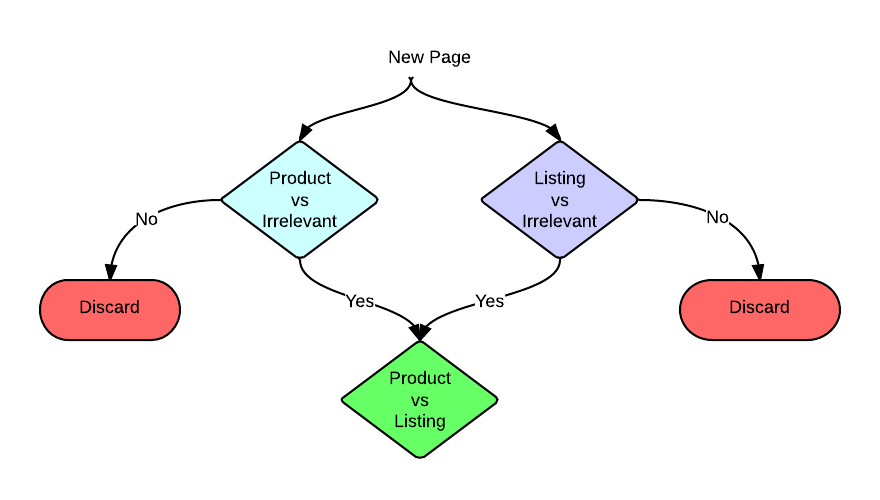
\includegraphics[scale=0.4]{binclass}
\end{figure}



\section{Experiments and Results}

The experiments were performed using a 10-fold cross validation method
and the model that gave the best performance on the validation set
was selected. The performance measures used were f-measure for approach
1 and AUC-ROC, Accuracy for approach 2. The 

\begin{table}[H]
\begin{centering}
\caption{Approach 1 - One Class SVMs with the indicated positive class}

\par\end{centering}

\centering{}%
\begin{tabular}{|c|c|c|c|}
\hline 
\textbf{Positive class} & \textbf{Precision} & \textbf{Recall } & \textbf{f-Measure}\tabularnewline
\hline 
\textbf{Product Page Classifier} & 0.5 & 0.09 & 0.16\tabularnewline
\hline 
\textbf{Listing Page Classifier} & 0.71 & 0.049 & 0.58\tabularnewline
\hline 
\end{tabular}
\end{table}


As discussed above, the outlier approach performs poorly while differentiating
irrelevant pages from product pages. Hence, we need to treat the irrelevant
pages as a third class. The following results show the improvement
that happens as a result of using binary classifiers.

\begin{table}[H]
\begin{centering}
\caption{Approach 2 - SVM results}

\par\end{centering}

\centering{}%
\begin{tabular}{|c|c|c|c|c|}
\hline 
\multirow{2}{*}{\textbf{Classifier}} & \multicolumn{2}{c|}{\textbf{Train Data }} & \multicolumn{2}{c|}{\textbf{Test Data}}\tabularnewline
\cline{2-5} 
 & \textbf{AUC-ROC} & \textbf{Accuracy} & \textbf{AUC-ROC} & \textbf{Accuracy}\tabularnewline
\hline 
\textbf{Product vs Irrelevant} & 0.99 & 0.99 & 0.66 & 0.64\tabularnewline
\hline 
\textbf{Listing vs Irrelevant} & 0.99 & 0.99 & 0.78 & 0.65\tabularnewline
\hline 
\textbf{Product vs Listing} & 0.99 & 0.99 & 0.81 & 0.76\tabularnewline
\hline 
\end{tabular}
\end{table}


\begin{table}[H]
\begin{centering}
\caption{Approach 2 - Maximum Entropy classification results}

\par\end{centering}

\centering{}%
\begin{tabular}{|c|c|c|c|c|}
\hline 
\multirow{2}{*}{\textbf{Classifier}} & \multicolumn{2}{c|}{\textbf{Train Data }} & \multicolumn{2}{c|}{\textbf{Test Data}}\tabularnewline
\cline{2-5} 
 & \textbf{AUC-ROC} & \textbf{Accuracy} & \textbf{AUC-ROC} & \textbf{Accuracy}\tabularnewline
\hline 
\textbf{Product vs Irrelevant} & 0.94 & 0.88 & 0.91 & 0.86\tabularnewline
\hline 
\textbf{Listing vs Irrelevant} & 0.89 & 0.84 & 0.88 & 0.83\tabularnewline
\hline 
\textbf{Product vs Listing} & 0.95 & 0.90 & 0.93 & 0.89\tabularnewline
\hline 
\end{tabular}
\end{table}


\begin{table}[H]
\begin{centering}
\caption{Approach 2 - Random Forest results}

\par\end{centering}

\centering{}%
\begin{tabular}{|c|c|c|c|c|}
\hline 
\multirow{2}{*}{\textbf{Classifier}} & \multicolumn{2}{c|}{\textbf{Train Data }} & \multicolumn{2}{c|}{\textbf{Test Data}}\tabularnewline
\cline{2-5} 
 & \textbf{AUC-ROC} & \textbf{Accuracy} & \textbf{AUC-ROC} & \textbf{Accuracy}\tabularnewline
\hline 
\textbf{Product vs Irrelevant} & 1 & 0.99 & 0.98 & 0.93\tabularnewline
\hline 
\textbf{Listing vs Irrelevant} & 0.99 & 0.99 & 0.93 & 0.90\tabularnewline
\hline 
\textbf{Product vs Listing} & 1 & 0.99 & 0.99 & 0.95\tabularnewline
\hline 
\end{tabular}
\end{table}


\begin{table}[H]
\begin{centering}
\caption{Approach 2 - Gradient Boosting results}

\par\end{centering}

\centering{}%
\begin{tabular}{|c|c|c|c|c|}
\hline 
\multirow{2}{*}{\textbf{Classifier}} & \multicolumn{2}{c|}{\textbf{Train Data }} & \multicolumn{2}{c|}{\textbf{Test Data}}\tabularnewline
\cline{2-5} 
 & \textbf{AUC-ROC} & \textbf{Accuracy} & \textbf{AUC-ROC} & \textbf{Accuracy}\tabularnewline
\hline 
\textbf{Product vs Irrelevant} & 0.97 & 0.92 & 0.96 & 0.99\tabularnewline
\hline 
\textbf{Listing vs Irrelevant} & 0.97 & 0.94 & 0.92 & 0.90\tabularnewline
\hline 
\textbf{Product vs Listing} & 0.98 & 0.93 & 0.97 & 0.91\tabularnewline
\hline 
\end{tabular}
\end{table}



\section{Conclusions and Future Work}

The biggest challenge in the problem was to differentiate between
product pages and product listing pages, due to the large overlap
in the content of the two classes. Like poduct pages, the product
listing pages themselves may contain short descriptions of a number
of products. Hence, content specific features alone are not sufficient
to differentiate between the two classes. By integrating structural
features along with the text features, we were able to obtain sets
of classifiers that differentiate between each of the avalable classes.
These can be merged into one ensemble classifier and used along with
a web crawler to eliminate a number of unwanted pages, thereby reducing
the load on the crawler.

Our main aim was to compare how the classifiers behave when trained
with different sets of features. We tried content-based features,
structure based features and a combination of both. If we use content
only, we can eliminate irrelevant pages with a good score, but it
is difficult to differentiate between product and listing pages. Similarly,
for structure based features, it will be difficult to differentiate
between product and irrelevant pages. However, one advantage of using
structure based features is that they are universal for all webpages.
We can randomly take out some pages from http://www.amazon.cn , the
Chinese website of Amazon and attempt to classify. It is expected
to give a good performance as the structure remains the same irrespective
of the content. 

Another set of features, that can be used are those obtained from
the URLs. Using URL based features for Web Page Classification \cite{g}
can be very beneficial as they are easy to train and might contain
vital information including the title of the page. In our case, we
could observe that several product page URLs had a pattern like ‘……?productId=xxxxx….’.
However, due to the vast diversity of retail pages it was not possible
to train a reasonable classifier based on these features.
\begin{thebibliography}{1}
\bibitem[1]{f} Arasu, A., Garcia-Molna, H.: Extracting structured
data from web pages. In: SIGMOD, pp. 337–348 (2003) 

\bibitem[7]{a}B. Schölkopf, R.C. Williamson, A.J. Smola, J.Shawe-Taylor
and J.C. Platt. Support Vector Method for Novelty Detection . Technical
report, Microsoft Research, MSR-TR-99-87, 1999.

\bibitem[2]{b} L. M. Manevitz and M. Yousef. One-class SVMs for document
classification. Journal of MachineLearning Research,2:139-154, 2001

\bibitem[3]{c} C.C. Chang and C. J. Lin. LIBSVM: A Library for Support
Vector Machines (2013) 

\bibitem[4]{d} L. Breiman. Random forests. Machine Learning, 45(1):
5–32, 2001. 1

\bibitem[6]{g} An Experiment to Test URL Features for Web Page Classification,
Inma Hern´andez,Carlos R. Rivero, David Ruiz, and Jos´e Luis Arjona 

\bibitem[5]{e} Christopher D. Manning and Hinrich Schutze: Foundations
of Statistical Natural Language Processing (1999)\end{thebibliography}

\end{document}
